\documentclass{article}
 \usepackage{tikz}
 \usepackage{xcolor}
 \usetikzlibrary{matrix,decorations.pathreplacing, calc, positioning}
 
 \definecolor{syntagmaticaxiscolor}{RGB}{0,32,96}
  \definecolor{paradigmaticaxiscolor}{RGB}{96,32,0}

 \begin{document}

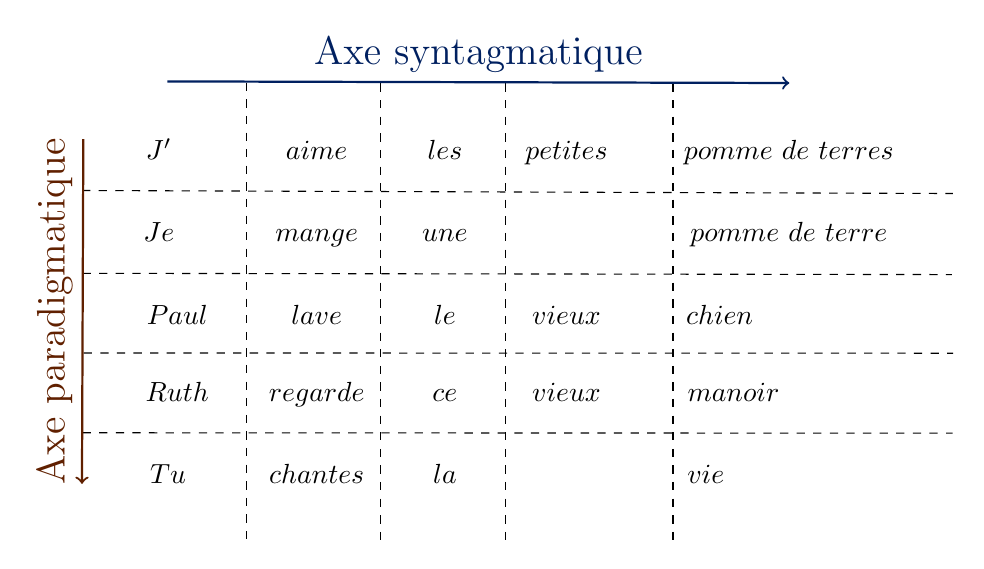
\begin{tikzpicture}
\matrix [
	matrix of math nodes,
	%left delimiter=,
	%right delimiter=,
	row sep=0.5cm,  %row sep=-\pgflinewidth
	column sep=0.5cm,
	nodes in empty cells
	] (m) {
J'~~~~& aime        & les  & petites & ~~pomme~de~terres \\
Je~~~~& mange   & une &            & ~~pomme~de~terre \\
Paul     & lave       & le     & vieux  & ~~chien~~~~~~~~~~~~~~~ \\ 
Ruth    & regarde  & ce    & vieux  & ~~manoir ~~~~~~~~~~~~\\
Tu ~~  & chantes  & la     &            & ~~vie ~~~~~~~~~~~~~~~~~~\\};


 
%\draw[dashed] ($0.5*(m-3-1.south west)+0.5*(m-4-1.north west)$) --
 %($0.5*(m-1-5.south east)+0.5*(m-1-6.north east)$);

\node[above=10pt of m-1-1] (top-1) {$$};
\node[above=10pt of m-1-2] (top-2) {$$};
\node[above=10pt of m-1-3] (top-3) {$$};
\node[above=10pt of m-1-4] (top-4) {$$};
\node[above=10pt of m-1-5] (top-5) {$$};

\node[below=10pt of m-5-1] (bot-1) {$$};
\node[below=10pt of m-5-2] (bot-2) {$$};
\node[below=10pt of m-5-3] (bot-3) {$$};
\node[below=10pt of m-5-4] (bot-4) {$$};
\node[below=10pt of m-5-5] (bot-5) {$$};

\node[left=12pt of m-1-1] (left-1) {$$};
\node[left=12pt of m-2-1] (left-2) {$$};
\node[left=12pt of m-3-1] (left-3) {$$};
\node[left=12pt of m-4-1] (left-4) {$$};
\node[left=14pt of m-5-1] (left-5) {$$};

\node[right=12pt of m-1-5] (right-1) {$$};
\node[right=12pt of m-2-5] (right-2) {$$};
\node[right=12pt of m-3-5] (right-3) {$$};
\node[right=12pt of m-4-5] (right-4) {$$};
\node[right=12pt of m-5-5] (right-5) {$$};

% Horizontal dashes
\draw[dashed] ($0.5*(left-1.south west)+0.5*(left-2.north west)$) -- ($0.5*(right-1.south east)+0.5*(right-2.north east)$);
\draw[dashed] ($0.5*(left-2.south west)+0.5*(left-3.north west)$) -- ($0.5*(right-2.south east)+0.5*(right-3.north east)$);
\draw[dashed] ($0.5*(left-3.south west)+0.5*(left-4.north west)$) -- ($0.5*(right-3.south east)+0.5*(right-4.north east)$);
\draw[dashed] ($0.5*(left-4.south west)+0.5*(left-5.north west)$) -- ($0.5*(right-4.south east)+0.5*(right-5.north east)$);

% Vertical dashes
\draw[dashed] ($0.5*(top-1.north east)+0.5*(top-2.north west)$) -- ($0.5*(bot-1.south east)+0.5*(bot-2.south west)$);
\draw[dashed] ($0.5*(top-2.north east)+0.5*(top-3.north west)$) -- ($0.5*(bot-2.south east)+0.5*(bot-3.south west)$);
\draw[dashed] ($0.5*(top-3.north east)+0.5*(top-4.north west)$) -- ($0.5*(bot-3.south east)+0.5*(bot-4.south west)$);
\draw[dashed] ($0.5*(top-4.north east)+0.5*(top-5.north west)$) -- ($0.5*(bot-4.south east)+0.5*(bot-5.south west)$);


\draw[syntagmaticaxiscolor, ->,thick] (top-1.north west) -- (top-5.north east) node [pos=0.5,above,font=\Large] {Axe~syntagmatique};
\draw[paradigmaticaxiscolor, ->,thick] (left-1.north west) -- (left-5.south west) node [pos=0.5,above,font=\Large, rotate=90] {Axe~paradigmatique};


%\node[rectangle,left delimiter=\{] (del-left-2) at ($0.5*(left-4.east) +0.5*(left-6.east)$) {\tikz{\path (left-4.north east) rectangle (left-6.south west);}};
%\node[left=10pt] at (del-left-2.west) {$E_2$};

\end{tikzpicture}


  \end{document}